\documentclass{article}

% The official Overleaf template loads this package from the template project:
% https://github.com/ICLR/Master-Template/tree/master/iclr2025
\usepackage{iclr2025_conference,times}

\usepackage{hyperref}
\usepackage{url}
\usepackage{booktabs}
\usepackage{amsmath}
\usepackage{amssymb}
\usepackage{graphicx}
\usepackage{tikz}
\usetikzlibrary{arrows.meta,positioning,fit}

\title{Progress Report: Channel-Gated Partial Convolution for FasterNet}

\author{
Erkani Mert Tosun \\
Department of Computer Engineering \\
Hacettepe University \\
\texttt{N25123091}
}

% Uncomment for final/camera-ready formatting if requested by the instructor.
\iclrfinalcopy

\begin{document}

\maketitle

\begin{abstract}
This progress report studies an extension of FasterNet, a latency-oriented convolutional neural network family built around partial convolution (PConv). The original method argues that reducing floating point operations (FLOPs) is not sufficient for obtaining fast neural networks, because actual latency also depends on hardware utilization and floating point operations per second (FLOPS). FasterNet improves this utilization by applying spatial convolution only to a subset of feature channels and using pointwise convolution for cross-channel mixing. The proposed extension adds a lightweight Channel Gate Module (CGM) after PConv in each FasterNet block. The goal is to selectively recalibrate the spatially processed channels before pointwise mixing, while keeping the memory-access advantage of PConv mostly intact. The planned experiments compare vanilla FasterNet-T0/T1 and channel-gated variants on CIFAR-100 and Tiny-ImageNet using accuracy, parameter count, FLOPs, CPU/GPU latency, and gate-weight visualizations.
\end{abstract}

\section{Problem Definition}

Modern computer vision models must balance predictive accuracy with computational efficiency. This balance is especially important for edge devices, mobile applications, robotics, and real-time perception systems, where inference latency and memory bandwidth can be as important as top-1 accuracy. A common design principle in efficient convolutional neural networks is to reduce the number of FLOPs. For example, depthwise convolution separates spatial filtering from channel mixing and can dramatically lower the theoretical arithmetic cost of a convolutional block. However, the central observation of FasterNet is that low FLOPs do not automatically imply low latency \citep{chen2023fasternet}. Hardware speed depends not only on how many operations are executed, but also on how efficiently these operations are scheduled and how much memory movement is required.

The project problem is therefore: how can we improve or extend a latency-efficient convolutional backbone without destroying the computational properties that make it fast? More specifically, this project investigates whether PConv-based FasterNet blocks can benefit from explicit channel recalibration after spatial mixing. In the original FasterNet block, PConv applies a $3 \times 3$ convolution to only a fraction of the channels and leaves the remaining channels unchanged. Then a pointwise MLP mixes information across all channels. This design is fast, but it treats all spatially processed channels uniformly. In practice, different channels may capture edges, textures, object parts, or background patterns with different usefulness for the current input image. The proposed extension tests whether a small channel gate can emphasize informative PConv channels and suppress less useful ones before the following pointwise convolution.

The main challenges are as follows. First, any added module must be very lightweight; otherwise the extension may improve accuracy but contradict the motivation of FasterNet. Second, latency must be measured directly rather than inferred only from FLOPs, because the paper itself shows that FLOPs can be misleading. Third, training full ImageNet-scale FasterNet models is computationally expensive for a course project, so the experimental setting must be reduced without making the comparison meaningless. Finally, because the proposed gate is input-dependent, the project should not only report final accuracy but also analyze whether the learned gates behave in an interpretable and stable way.

\section{Related Work}

\subsection{Efficient convolutional networks}

Early efficient CNN families mainly focused on reducing arithmetic cost. MobileNetV1 introduced depthwise separable convolution, decomposing a standard convolution into a depthwise spatial convolution and a pointwise $1 \times 1$ convolution \citep{howard2017mobilenets}. MobileNetV2 further improved this design using inverted residual blocks and linear bottlenecks \citep{sandler2018mobilenetv2}. ShuffleNet and ShuffleNetV2 targeted efficient inference under mobile constraints by combining grouped pointwise convolutions, channel shuffle operations, and practical design guidelines for low-latency networks \citep{zhang2018shufflenet,ma2018shufflenetv2}. EfficientNet later used compound scaling to jointly increase depth, width, and resolution under a fixed resource budget \citep{tan2019efficientnet}.

These methods established the importance of compact architecture design, but they also show a limitation of FLOP-centered optimization. Depthwise convolution has few operations, yet it can suffer from poor hardware utilization because it performs many memory accesses relative to computation. ShuffleNetV2 explicitly notes that fragmentation, element-wise operations, and memory access cost can strongly affect real speed \citep{ma2018shufflenetv2}. FasterNet continues this line of reasoning by directly optimizing for high effective FLOPS, meaning that a model should keep hardware arithmetic units busy rather than only minimizing the operation count.

\subsection{Modern convolutional backbones}

Although vision transformers changed the design landscape, modern CNNs remain competitive when carefully designed. ConvNeXt revisited standard ConvNet components and showed that convolutional networks can match transformer-era performance when modern training recipes and architectural choices are used \citep{liu2022convnext}. FasterNet is related to this renewed interest in strong convolutional backbones, but it focuses more directly on latency. Its core block keeps a simple convolutional structure and uses PConv to reduce memory access cost while preserving spatial feature extraction.

\subsection{Attention and channel recalibration}

The proposed extension is inspired by channel attention modules. Squeeze-and-Excitation Networks (SENet) introduced a lightweight mechanism that globally pools feature maps, passes the channel descriptor through a bottleneck MLP, and uses a sigmoid gate to rescale channels \citep{hu2018senet}. CBAM extended this idea with both channel and spatial attention \citep{woo2018cbam}. These modules often improve accuracy by allowing a network to adaptively emphasize useful features for each input.

However, the proposed CGM is not a direct insertion of a generic attention block into FasterNet. The key difference is placement and scope. Applying attention to all channels after every block could introduce unnecessary overhead and weaken the latency motivation. Instead, CGM operates only on the subset of channels processed by PConv. This makes the extension more aligned with FasterNet's design principle: improve the informativeness of the spatially mixed channels while avoiding expensive global modification of the whole block.

\section{Method}

\subsection{Base method: FasterNet and partial convolution}

FasterNet is built around the observation that a neural network should be evaluated not only by FLOPs but also by its achieved computational throughput. A standard convolution performs spatial mixing for every input channel and every output channel, which is accurate but expensive. Depthwise convolution reduces FLOPs by applying spatial filtering independently per channel, but in many architectures this requires increasing width to recover accuracy. Wider layers increase memory traffic, and the resulting model may have low actual FLOPS.

PConv offers a different trade-off. Given an input tensor $X \in \mathbb{R}^{B \times C \times H \times W}$, the channels are split into two parts:
\begin{equation}
X = [X_p, X_u],
\end{equation}
where $X_p$ contains $C_p = C / n$ channels and $X_u$ contains the remaining untouched channels. PConv applies a $3 \times 3$ convolution only to $X_p$:
\begin{equation}
\hat{X}_p = \mathrm{Conv}_{3 \times 3}(X_p),
\end{equation}
and then concatenates the result with $X_u$:
\begin{equation}
\hat{X} = [\hat{X}_p, X_u].
\end{equation}
The following pointwise convolutional MLP mixes information across channels. In the official FasterNet implementation, the main block applies PConv as spatial mixing, then a two-layer pointwise MLP with normalization and activation, and finally adds the residual shortcut.

\begin{figure}[t]
\centering
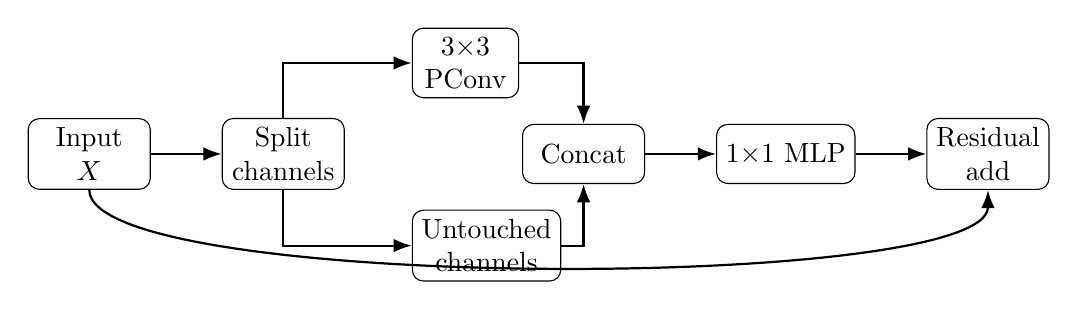
\begin{tikzpicture}[
    node distance=0.9cm,
    block/.style={draw, rounded corners, align=center, minimum height=0.75cm, minimum width=1.55cm},
    smallblock/.style={draw, rounded corners, align=center, minimum height=0.65cm, minimum width=1.35cm},
    arrow/.style={-Latex, thick}
]
\node[block] (x) {Input\\$X$};
\node[block, right=of x] (split) {Split\\channels};
\node[smallblock, above right=0.25cm and 0.85cm of split] (pconv) {$3{\times}3$\\PConv};
\node[smallblock, below right=0.25cm and 0.85cm of split] (id) {Untouched\\channels};
\node[block, right=2.25cm of split] (concat) {Concat};
\node[block, right=of concat] (mlp) {$1{\times}1$ MLP};
\node[block, right=of mlp] (add) {Residual\\add};
\draw[arrow] (x) -- (split);
\draw[arrow] (split) |- (pconv);
\draw[arrow] (split) |- (id);
\draw[arrow] (pconv) -| (concat);
\draw[arrow] (id) -| (concat);
\draw[arrow] (concat) -- (mlp);
\draw[arrow] (mlp) -- (add);
\draw[arrow] (x.south) .. controls +(0,-1.3) and +(0,-1.3) .. (add.south);
\end{tikzpicture}
\caption{Simplified FasterNet block. PConv performs spatial mixing on only a subset of channels, while the pointwise MLP performs channel mixing.}
\label{fig:base_block}
\end{figure}

\subsection{Proposed extension: Channel Gate Module}

The proposed extension adds a Channel Gate Module immediately after the PConv operation. Instead of recalibrating all $C$ channels, the gate is applied only to the $C_p$ channels that were spatially processed. Let $\hat{X}_p \in \mathbb{R}^{B \times C_p \times H \times W}$ be the PConv output. CGM first computes a global average pooled descriptor:
\begin{equation}
z_c = \frac{1}{HW}\sum_{i=1}^{H}\sum_{j=1}^{W} \hat{X}_{p,c,i,j}.
\end{equation}
The descriptor is passed through a bottleneck MLP:
\begin{equation}
g = \sigma(W_2 \delta(W_1 z)),
\end{equation}
where $\delta$ is ReLU, $\sigma$ is sigmoid, $W_1 \in \mathbb{R}^{C_p/r \times C_p}$, $W_2 \in \mathbb{R}^{C_p \times C_p/r}$, and $r$ is a reduction ratio such as $4$. The gated PConv output is:
\begin{equation}
\tilde{X}_{p,c,:,:} = g_c \cdot \hat{X}_{p,c,:,:}.
\end{equation}
Finally, $\tilde{X}_p$ is concatenated with the untouched channels and passed to the original pointwise MLP.

\begin{figure}[t]
\centering
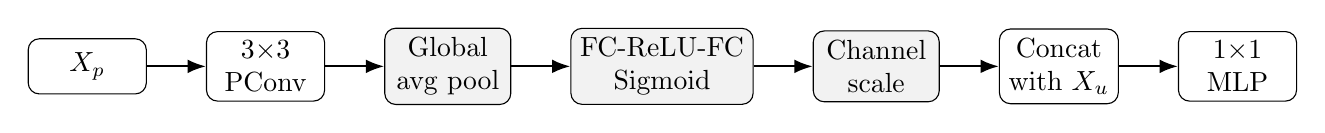
\begin{tikzpicture}[
    node distance=0.75cm,
    block/.style={draw, rounded corners, align=center, minimum height=0.7cm, minimum width=1.5cm},
    gate/.style={draw, rounded corners, align=center, minimum height=0.7cm, minimum width=1.6cm, fill=gray!10},
    arrow/.style={-Latex, thick}
]
\node[block] (xp) {$X_p$};
\node[block, right=of xp] (pconv) {$3{\times}3$\\PConv};
\node[gate, right=of pconv] (gap) {Global\\avg pool};
\node[gate, right=of gap] (fc) {FC-ReLU-FC\\Sigmoid};
\node[gate, right=of fc] (scale) {Channel\\scale};
\node[block, right=of scale] (cat) {Concat\\with $X_u$};
\node[block, right=of cat] (pw) {$1{\times}1$\\MLP};
\draw[arrow] (xp) -- (pconv);
\draw[arrow] (pconv) -- (gap);
\draw[arrow] (gap) -- (fc);
\draw[arrow] (fc) -- (scale);
\draw[arrow] (scale) -- (cat);
\draw[arrow] (cat) -- (pw);
\end{tikzpicture}
\caption{Proposed Channel Gate Module. The gate is restricted to the PConv-processed channel subset, limiting overhead while allowing input-adaptive channel recalibration.}
\label{fig:cgm}
\end{figure}

\subsection{Planned variants}

The project will evaluate multiple variants to separate the effect of the gate from general training noise. The baseline is vanilla FasterNet-T0/T1. The main proposed model applies CGM after every PConv block. Two ablations apply CGM selectively to early stages and late stages. Early-stage gates may help low-level edge and texture features, while late-stage gates may help semantic feature selection. A final ablation changes the reduction ratio $r$ to test the trade-off between expressiveness and overhead.

\begin{table}[t]
\caption{Planned model variants.}
\label{tab:variants}
\centering
\begin{tabular}{lll}
\toprule
Variant & CGM placement & Purpose \\
\midrule
FasterNet baseline & None & Reference accuracy and latency \\
CGM-All & Stages 1--4 & Main proposed extension \\
CGM-Early & Stages 1--2 & Low-level feature recalibration \\
CGM-Late & Stages 3--4 & High-level semantic recalibration \\
CGM-r & All stages, varying $r$ & Overhead/accuracy trade-off \\
\bottomrule
\end{tabular}
\end{table}

\section{Experimental Settings and Preliminary Results}

\subsection{Datasets}

The original FasterNet paper reports ImageNet-1K classification results. For this course project, full ImageNet training is not realistic due to time and hardware constraints. Therefore, the planned datasets are CIFAR-100 and Tiny-ImageNet. CIFAR-100 contains 60,000 images from 100 classes, with 50,000 training images and 10,000 test images. The images are $32 \times 32$, so the FasterNet configuration must be adjusted or images must be resized to match the patch embedding design. Tiny-ImageNet contains 200 classes with $64 \times 64$ images, providing a more challenging setting while remaining much smaller than ImageNet-1K.

\subsection{Implementation environment}

The official FasterNet repository is implemented in PyTorch and PyTorch Lightning. The repository dependencies specify Python 3.9.12, PyTorch 1.11.0, torchvision 0.12.0, PyTorch Lightning 1.6.5, timm 0.6.5, and fvcore for FLOP/parameter measurement. Preliminary code inspection shows that the original data pipeline supports ImageNet-style folders by default. Therefore, an implementation step of this project is to add CIFAR-100 and Tiny-ImageNet datamodules or to adapt these datasets into an ImageFolder-compatible directory structure.

\subsection{Training protocol}

The initial training plan is to use FasterNet-T0 as the primary model and FasterNet-T1 as a secondary model if time and hardware allow. Since the goal is not to reproduce full ImageNet performance, the experiments will use moderate training schedules. A planned CIFAR-100 setting is AdamW optimization, cosine learning-rate decay, batch size between 128 and 256 depending on GPU memory, 100--200 epochs, label smoothing, random crop, horizontal flip, and optional MixUp/CutMix if stable. Tiny-ImageNet will use similar augmentation with input resolution 64 or resized 224 depending on the final architecture configuration. All compared variants will use the same training settings.

\subsection{Evaluation metrics}

The primary predictive metric is top-1 classification accuracy. Efficiency will be evaluated using parameter count, FLOPs, and measured latency. FLOPs and parameter count will be computed with fvcore, matching the official repository utilities. Latency will be measured directly using repeated forward passes after warm-up, separately for CPU and GPU if available. The report will emphasize direct latency because FasterNet's main argument is that FLOPs alone can be misleading.

For interpretability, the gate values produced by CGM will be collected across layers and images. The planned visualizations include mean gate activation per block, gate-value histograms, and comparisons between correctly and incorrectly classified examples. These visualizations are intended to answer whether CGM learns meaningful channel preferences or simply converges to nearly constant scaling.

\subsection{Preliminary status}

At the time of this progress report, the project has completed paper selection, extension design, repository inspection, and experimental planning. The official implementation has a clean insertion point for the proposed extension: the \texttt{MLPBlock} applies \texttt{Partial\_conv3} before the pointwise MLP, so CGM can be added immediately after the spatial mixing step. The main engineering work that remains is dataset support and experiment execution.

\begin{table}[t]
\caption{Current progress and expected next steps.}
\label{tab:progress}
\centering
\begin{tabular}{lll}
\toprule
Component & Status & Notes \\
\midrule
Paper and repository selection & Completed & FasterNet official PyTorch code selected \\
Extension design & Completed & CGM after PConv on processed channels \\
Dataset pipeline & In progress & Need CIFAR-100/Tiny-ImageNet support \\
Baseline training & Planned & FasterNet-T0 first, T1 if feasible \\
CGM implementation & Planned & Minimal changes to FasterNet block \\
Latency/FLOP analysis & Planned & Use official fvcore and latency utilities \\
Gate visualization & Planned & Save and plot gate activations \\
\bottomrule
\end{tabular}
\end{table}

No final numerical training results are reported yet. This is intentional: the current stage is a progress report, and the next milestone is to obtain a verified FasterNet-T0 baseline on CIFAR-100. After the baseline is stable, the same training script will be used for CGM variants so that any performance difference is attributable to the proposed extension rather than to mismatched experimental settings.

\section{Expected Contribution}

The expected contribution is a small but focused extension of FasterNet that tests whether channel recalibration can improve the usefulness of PConv features without eliminating the speed advantage of partial convolution. Even if the final accuracy gain is modest, the project can still provide useful evidence by reporting the accuracy-overhead trade-off, stage-wise ablation results, and gate visualizations. This makes the project more informative than a simple accuracy comparison, because it directly investigates the design tension identified by the original paper: fast models must consider both computation and memory behavior.

\bibliography{references}
\bibliographystyle{iclr2025_conference}

\end{document}
